\input ../SlidePreamble
\input ../preamble

\newcommand{\solution}[1]{\bigskip {\bf Solution}: #1}

\begin{document}

{\Huge
  \centerline{\bf TTIC 31230, Fundamentals of Deep Learning}
  \bigskip
  \centerline{David McAllester, Winter 2019}
  \vfill
  \centerline{\bf Stochastic Gradient Descent (SGD)}
  \vfill
  \vfill
  \centerline{Gradient Flow and Langevin Dynamics}
  \vfill

\slide{Gradient Flow}

Gradient flow is a non-stochastic ({\color{red} deterministic}) model of {\color{red} stochastic} gradient descent (SGD).

\vfill
Gradient flow is defined by the {\color{red} total gradient} differential equation

$${\color{red} \frac{d \Phi}{d t} = - g(\Phi) \;\;\;\;\;\; g(\Phi) = \nabla_\Phi\; E_{(x,y) \sim \mathrm{Train}}\;{\cal L}(\Phi,x,y)}$$

\vfill
We let $\Phi(t)$ be the solution satisfying $\Phi(0) = \Phi_{\mathrm{init}}$.

\slide{Gradient Flow}
$${\color{red} \frac{d \Phi}{d t} = - g(\Phi)}$$

\vfill
For small values of $\Delta t$ this differential equation can be approximated by

\vfill
$${\color{red} \Delta \Phi = - g(\Phi)\Delta t}$$

\vfill
Here $\Delta t$ can be interpreted as a learning rate.

\slide{Gradient Flow also Models SGD}
Consider the SGD update with $\hat{g}$ from a random data point


{\color{red} $$\Delta \Phi = - \hat{g}\Delta t$$}

\vfill
This also converges to deterministic gradient flow as $\Delta t$ goes to zero.

\vfill
To see this note that we can divide the updates into $\sqrt{N}$ blocks each of size $\sqrt{N}$.  The ``time'' spent within each block is $t/\sqrt{N}$ which converges to 0.
But the number of updates within each block grows as $\sqrt{N}$ and hence the average update within a block converges to $g$.

\slide{Gradient Flow also Models SGD}
Consider the SGD update with $\hat{g}$ from a random data point


{\color{red} $$\Delta \Phi = - \hat{g}\Delta t$$}

\vfill
The sum of the learning rates can be interpreted as ``time''.

\slide{MCMC models of SGD}

\centerline{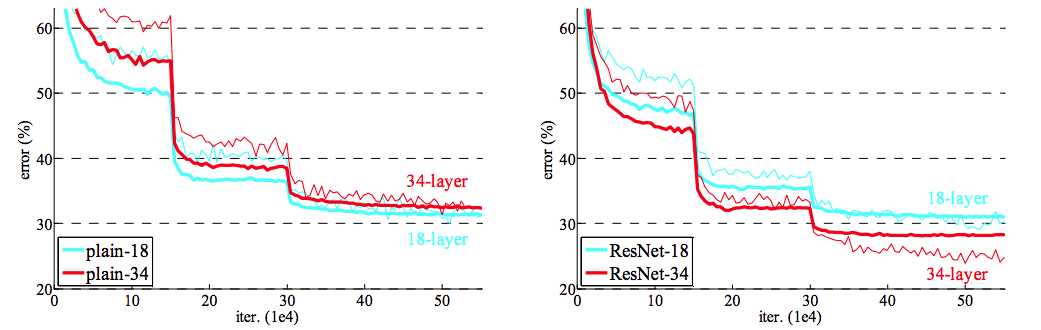
\includegraphics[width = 7in]{../images/annealing}}

\vfill
These Plots are from the original ResNet paper.  Left plot is for CNNs without residual skip connections, the right plot is ResNet.

\vfill
Thin lines are training error, thick lines are validataion error.

\vfill
In all cases $\eta$ is reduced twice, each time by a factor of 2.

\slide{Converged Loss as a Function of $\eta$}

\centerline{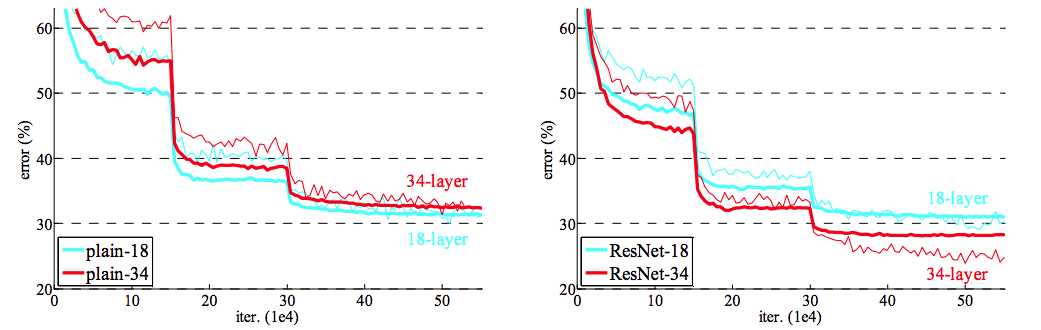
\includegraphics[width = 4in]{../images/annealing}}
For each value of $\eta$ we converge at a loss ${\cal L}(\eta)$.
\begin{eqnarray*}
{\cal L}(0) & \doteq & \lim_{\eta \rightarrow 0}\;{\cal L}(\eta) \\
\\
& = & {\cal L}(\Phi^*)\;\;\;\;\mbox{$\Phi^*$ a local optimum}
\end{eqnarray*}

\vfill
Can we do a Taylor expansion of ${\cal L}(\eta)$?
$${\cal L}(\eta) = {\cal L}(\Phi^*) + \left(\left.\frac{d{\cal L}}{d \eta}\right|_{\eta = 0}\right)\eta + \ldots$$

\slide{A Nice Theorem (TZ)}
$${\cal L}(\eta) = {\cal L}(\Phi^*) + \left(\left.\frac{d{\cal L}}{d \eta}\right|_{\eta = 0}\right)\eta + \ldots$$

\vfill
Let $i$ index a training example and let $g_i$ denote $\nabla_\Phi {\cal L}_i(\Phi)$ at $\Phi = \Phi^*$.

\vfill
Theorem:
$${\color{red} \left.\frac{\partial {\cal L}(\eta)}{\partial \eta}\right|_{\eta = 0} \;\;=\;\; \frac{1}{4}\; E_i\; ||g_i||^2}$$

\slide{Proof Step 1 (TZ)}

\vfill
Let $i$ index a training example and let ${\cal L}_i(\Phi^* + \Delta \Phi)$ be the loss on training example $i$
with model parameters $\Phi^* + \Delta\Phi$. 

\vfill
We take a second order Taylor expansion.

\begin{eqnarray*}
{\cal L}(\Phi) & = & E_i\;{\cal L}_i(\Phi) \\
\\
{\cal L}_i(\Phi^* + \Delta \Phi) & = & {\cal L}_i + g_i \Delta \Phi + \frac{1}{2} \Delta\Phi^\top H_i \Delta\Phi \\
\\
E_i\; g_i & = & 0\\
\\
E_i\; H_i & & \mbox{is positive definite}
\end{eqnarray*}

\slide{Proof: Step 2 (TZ)}

\begin{eqnarray*}
{\cal L}(\eta) & = & \;\;\; E_{\Delta \Phi \sim P_\eta}\;E_i \;\;\;\; {\cal L}_i + g_i\Delta _\Phi + \frac{1}{2}\;\Delta \Phi^\top H_i \Delta \Phi \\
\\
& = & E_i\; {\cal L}_i + E_{\Delta \Phi \sim P_\eta} \;\;\;\;(E_i\;g_i) \;\Delta \Phi + \frac{1}{2}\;\Delta \Phi^\top (E_i\; H_i) \Delta \Phi \\
\\
& = & {\cal L}(\Phi^*)\;\; + \;\; E_{\Delta \Phi \sim P_\eta}\;\;\;\frac{1}{2}\;\Delta \Phi^\top (E_i\;H_i) \Delta \Phi
\end{eqnarray*}

\slide{Proof: Step 3 (TZ)}
Because $P_\eta$ is a stationary distribution we must have

$$E_{\Delta \Phi \sim P_\eta}E_i\; ||\Delta \Phi - \eta (g_i + H_i\Delta \Phi)||^2 = E_{\Delta \Phi \sim P_\eta}\; ||\Delta \Phi||^2$$

\vfill
$$E_{\Delta \Phi \sim P_\eta}E_i\;-2\eta \Delta \Phi^\top (g_i + H_i\Delta \Phi) +\eta^2||(g_i + H_i\Delta \Phi)||^2 = 0$$

\vfill
$$E_{\Delta \Phi \sim P_\eta}\;\left(\frac{1}{2}\Delta \Phi^\top (E_i \;H_i)\Delta \Phi\right) = \frac{\eta}{4}\;E_{\Delta \Phi \sim P_\eta}E_i \;||(g_i + H_i\Delta \Phi)||^2$$

\vfill
$${\color{red} {\cal L}(\eta)  = {\cal L}(\Phi^*) + \frac{\eta}{4}\;E_{\Delta \Phi \sim P_\eta}E_i \;||(g_i + H_i\Delta \Phi)||^2}$$

\slide{Proof Step 4 (TZ)}

\begin{eqnarray*}
{\color{red} {\cal L}(\eta)}  & {\color{red} =} & {\color{red} {\cal L}(\Phi^*) + \frac{\eta}{4}\;E_{\Delta \Phi \sim P_\eta}E_i \;||(g_i + H_i\Delta \Phi)||^2} \\
\\
\\
{\color{red} \left.\frac{\partial {\cal L}(\eta)}{\partial \eta}\right|_{\eta = 0}} & = & \frac{1}{4} \; \lim_{\eta \rightarrow 0} \; E_{\Delta \Phi \sim P_\eta}\; E_i \;||(g_i + H_i\Delta \Phi)||^2 \\
\\
\\
& {\color{red} =} & {\color{red} \frac{1}{4}\; E_i\;||g_i||^2}
\end{eqnarray*}


\slide{Langevin Dynamics}

Can we analytically solve for stationary distributions?

\vfill
Is the stationary distributin some kind of Gibbs Distribution?

\vfill
Langevin dynamics models both the stationary distribution and non-stationary stochastic dynamics
with {\color{red} a continuous time stochastic differential equation}.

\slide{Langevin Dynaimcs}


\vfill
Consider SGD with $B = 1$.

$$\Phi \;\minuseq\; \eta\hat{g}$$

\vfill
For $N$ steps of SGD we define $\Delta t = N \eta$.

\vfill
In Langevin dynamics we hold $\eta > 0$ fixed.

\vfill
We then consider $\Delta t$ large compared to $\eta$ (so that it corresponds to many SGD updates) but
small enough so that the gradient distribution does not change during the interval $\Delta t$.

\slide{Langevin Dynamics}

If the mean gradient $g(\Phi)$ is approximately constant over the interval $\Delta t = N \eta$ we have

$$\Phi(t + \Delta t)  \approx \Phi(t) -g(\Phi)\Delta t + \eta \sum_{j=1}^N (g(\Phi) - \hat{g}_i)$$

\vfill
The Random variables in the last term have zero mean.

\vfill
By the law of large numbers a sum (not the average) of $N$ random vectors will approximate a Gaussian distribution where the standard deviation
grows like $\sqrt{N}$.

\slide{Langevin Dynamics}

Let $\Sigma$ be the covariance matrix of the random variable $\hat{g}$ and assume this is approximately constant over the interval $\Delta t$.

\vfill
Let $\epsilon$ be a zero mean Gaussian random variable with the same covariance matrix $\Sigma$.

\begin{eqnarray*}
\Phi(t + \Delta t) & \approx & \Phi(t) -g(\Phi)\Delta t + \eta \sum_{j=1}^N (g(\Phi) - \hat{g}_i) \\
\\
& \approx & \Phi(t) -g(\Phi)\Delta t + \eta \epsilon \sqrt{N} \\
\\
& = & \Phi(t) -g(\Phi)\Delta t + \eta \epsilon \sqrt{\frac{\Delta t}{\eta}}
\end{eqnarray*}


\slide{Langevin Dynamics}

\begin{eqnarray*}
\Phi(t + \Delta t) & \approx & \Phi(t) -g(\Phi)\Delta t + \epsilon \sqrt{{\color{red} \eta}\Delta t}\;\;\;\;\;\; \epsilon \sim {\cal N}(0,\Sigma) \\
\\
& = & \Phi(t) -g(\Phi)\Delta t + \epsilon \sqrt{\Delta t}\;\;\;\;\;\; \epsilon \sim {\cal N}(0,{\color{red} \eta}\Sigma)
\end{eqnarray*}

\vfill
This can be modeled by a continuous time stochastic process --- Langevin dynamics --- defined by the notation

{\color{red} $$d\Phi =  -g(\Phi)dt + \epsilon \sqrt{dt}\;\;\;\;\;\; \epsilon \sim {\cal N}(0,\eta\Sigma)$$}

\vfill
This is a stochastic differential equation.

\vfill
If $g(\Phi) = 0$ and $\Sigma = I$ we get Brownian motion.

\slide{Langevin Dynamics}

\begin{eqnarray*}
\Phi(t + \Delta t) & \approx & \Phi(t) -g(\Phi)\Delta t + \epsilon\sqrt{\Delta t}\;\;\;\;\;\; \epsilon \sim {\cal N}(0,\eta\Sigma)
\end{eqnarray*}

\vfill
Note that for $\eta \rightarrow 0$ the noise term vanishes.  If we then take $\Delta t \rightarrow 0$ (at a slower rate) we are back to gradient flow.

\vfill
In Langevin dynamics we hold $\eta > 0 $ fixed.

\slide{Stationary Distributions}

SGD at $B = 1$ defines a Markov process

$$\Phi \;\minuseq \; \eta \hat{g}$$

\vfill
Under Langevin dynamics the stationary distribution is a continuous density in parameter space.

\vfill
If the covariance matrix is isotropic (all eigenvalues are the same) we get a Gibbs distribution.


\slide{The 1-D Langevin Stationary Distribution}

Consider SGD on a single parameter.

\vfill
Let $p$ be a probability density on $x$.

\vfill
Assume that the gradient $\hat{g}$ has variance $\sigma$ everywhere.

\vfill
There is a diffusion flow proportional to $\eta^2\sigma^2\;dp/dx$.

\vfill
There is a gradient flow equal to $\eta p \;d {\cal L}/dx$.

\vfill
For a stationary distribution the two flows cancel giving.

\vfill
{\color{red} $$\alpha \eta^2 \sigma^2 \frac{dp}{dx} = - \eta p\frac{d{\cal L}}{dx}$$}


\slide{The 1-D Langevin Stationary Distribution}

\vspace{-2ex}
\begin{eqnarray*}
\alpha \eta^2 \sigma^2 \frac{dp}{dx} & = & - \eta p\frac{d{\cal L}}{dx} \\
\\
\frac{dp}{p} & = & \frac{-d{\cal L}}{\alpha\eta\sigma^2} \\
\\
\ln p & = & \frac{-{\cal L}}{\alpha \eta \sigma^2} + C \\
\\
{\color{red} p(x)} & = & {\color{red} \frac{1}{Z}\exp\left(\frac{-{\cal L}(x)}{\alpha \eta \sigma^2}\right)}\;\;\alpha \approx 1/10
\end{eqnarray*}

\vfill
We get a Gibbs distribution!

\slide{A 2-D Langevin Stationary Distribution}

Let $p$ be a probability density on two parameters $(x,y)$.

\vfill
We consider the case where $x$ and $y$ are completely independent with
$${\cal L}(x,y) = {\cal L}(x) + {\cal L}(y)$$

\vfill
For completely independent variables we have
\begin{eqnarray*}
p(x,y) & = & p(x)p(y) \\
\\
&= & \frac{1}{Z} \exp\left(\frac{-{\cal L}(x)}{\alpha \eta \sigma_x^2} + \frac{-{\cal L}(y)}{\alpha \eta \sigma_y^2}\right)
\end{eqnarray*}

\slide{A 2-D Langevin Stationary Distribution}

\begin{eqnarray*}
p(x,y) & = & \frac{1}{Z} \exp\left(\frac{-{\cal L}(x)}{\alpha \eta \sigma_x^2} + \frac{-{\cal L}(y)}{\alpha \eta \sigma_y^2}\right) \\
\\
\\
& = & \frac{1}{Z} \exp\left(-\beta_x{\cal L}(x) - \beta_y{\cal L}(y)\right)
\end{eqnarray*}

\vfill
This is not a Gibbs distribution!

\vfill
It has two different temperature parameters!

\slide{Langevin and RMSProp}

Suppose we use parameter-specific learning rates $\eta_x$ and $\eta_y$

\begin{eqnarray*}
p(x,y) & = & \frac{1}{Z} \exp\left(\frac{-{\cal L}(x)}{\alpha \eta_x \sigma_x^2} + \frac{-{\cal L}(y)}{\alpha \eta_y \sigma_y^2}\right)
\end{eqnarray*}

Setting $\eta_x = \eta'/\sigma^2_x$ and $\eta_y = \eta'/\sigma^2_y$ gives

\begin{eqnarray*}
p(x,y) & = & \frac{1}{Z} \exp\left(\frac{-{\cal L}(x)}{\alpha \eta'} + \frac{-{\cal L}(y)}{\alpha \eta'}\right) \\
\\
& = & \frac{1}{Z} \exp\left(\frac{-{\cal L}(x,y)}{\alpha \eta'}\right)\;\;\;\mathrm{Gibbs!}
\end{eqnarray*}

\slide{Langevin and RMSProp}

Suppose we use parameter-specific learning rates $\eta_x$ and $\eta_y$

Setting $\eta_x = \eta'/\sigma^2_x$ and $\eta_y = \eta'/\sigma^2_y$ gives

\vfill
\begin{eqnarray*}
p(x,y) & = & \frac{1}{Z} \exp\left(\frac{-{\cal L}(x,y)}{\alpha \eta'}\right)\;\;\;\mathrm{Gibbs!}
\end{eqnarray*}

\vfill
RMSProp sets $\eta_x = \eta'/\sigma_x$ rather than $\eta_x = \eta'/\sigma_x^2$.  Empirically RMSProp seems better that the more
theoretically motivated algorithm.

\slide{END}
\end{document}
